\section{Code Sequential Rationales}

We present and describe \codeSeqRational: an approach designed to provide an automated and effective way to extract practical interpretability insights for NLM-based systems for code-related tasks. The approach \codeSeqRational is composed of three stages: \underline{A) Code Rationales:} Given a Neural Language Models (NLM) trained on a code-related task (\ie code completion, program repair, translation, or test generation), we rely on a proposed greedy algorithm know as \textit{sequence rationales} or \textit{greedy rationalization} \citep{vafa2021rationales} to understand NLM generation. Greedy rationalization finds the the minimum set of words that most contribute for the prediction of a specific token. In particular, for each token predicted by the NLM, greedy rationalization assigns rationales (numerical values organized in sets) to all input tokens or context window. \underline{B) Local post-hoc rationales:} Using a set of rationales to explain a single sample can be less informative if we operate over tokens without considering other code properties. That is the reason why we use \textit{human-interpretable concepts} to provide further understanding of a set of rationales for a single sample. Such concepts are obtained by using mapping functions or parser machines. And \underline{C) Global post-hoc rationales:} Once the set of rationales is aggregated for a single sample, we can escalate local post-hoc rationales methodology for whole sample set. By executing greedy rationalization on a sample set, we can observe a global behaviour of the NLM. 


\subsection{Code Rationales}
Rationales are subsets of input tokens from the context window that can \textit{explain} individual model predictions. By using combinatorial optimization, we are able to find the smallest subset of tokens that predict the same output as the full set of tokens. Such smallest subset are considered the best rationale. Vafa, et all introduce a strategy to approximate the \textit{best rationale} since enumerating all possible subsets is intractable. This strategy uses a greedy algorithm: \textit{greedy rationalization}. In order to use this greedy algorithm in any model, we must make the model "compatible" for a given combination of subsets of the input context. 

Consider the code sequence  $\mathcal{S} = w_{1:T}$, where the token $w_t$ is predicted given the context window $w_{<t}$ at any token position $t$. A sequence model $P_{\theta}$ is a probabilistic model that approximates a code generator $\mathcal{G}_c$ from samples $\mathcal{S}^n$, $n$ is the number of samples used for learning a model $p_{\theta}$. A code rational $r_w \subset w_{<t} $ is a subset of a context window $w_{<t}$ that can explain a prediction $w_t$.

The power set $\mathcal{R} = 2^{[t-1]}$ is the set of all possible subsets for the sequence context $w_{<t}$. The purpose of code rationales is to find a subset $r_w \in \mathcal{R}$ that achieves the same prediction as the context $w_{<t}$. Additionally, such rationales should be as smaller as possible $\hat{r_w}$ so that the interpretation of the token $w_t$ becomes as clearer as possible too. Take into consideration that predicting a token $w_t$ depends upon the context $w_{<t}$, while predicting a token $w'_t$ depends on the optimal rational $w_{r_w}$. Thus, code rationales are formulated as a combinatorial problem

\begin{equation}
r(w_{1:T}) = \arg \min_{r_w \in \mathcal{R}} |r| : \arg \max_{w'_t} P_{\theta}(w'_t|w_{r_w}) = w_t
\label{eq:combinatorial}
\end{equation}


Vafa et al., highlighted two main computational problems to solve objective function \equaref{eq:combinatorial}: 1) the optimization problem is intractable or NP-hard, and 2) evaluating conditioned distributions on subsets $w_r$ is also intractable over missing tokens. The first problem is solved by means of \textit{greedy rationalizations}, an algorithm to approximate a solution for \equaref{eq:combinatorial}. The second problem is solved using model \textit{compatibility}.

\textbf{Greedy rationalization} algorithm starts with the empty set adding iteratively the rationale that most contributes to the probability of $w_t$ at each step. Since the power set starts with the empty set 
$$r^{(0)}=\emptyset$$
the first rationale set is defined as
$$r^{(1)} = \arg \max_{j \in \{ [t-1] \} } P_{\theta}(w_t|w_j)$$
we can keep adding tokens to configure the rationale by choosing the sequence that maximizes the probability of the token $w_t$ at each step

\begin{equation}
r^{(k+1)} = r^{(k)} \cup  \arg \max_{j \in \{[t-1] \setminus r^{(k)} \} } P_{\theta}(w_t|w_{ \{ r^{(k)}\cup j \} })
\label{eq:greedy}
\end{equation}

The halting condition for the previous expression is, precisely, the \equaref{eq:combinatorial} when $ \arg \max_{w'_t} P_{\theta}(w'_t|w_{r^{(k)}}) = w_t$.  Note that a rational is the set of tokens that \textbf{covers} a given sequence $\mathcal{S}$ if such rational predicts a target token $w_t$. The algorithm described in Eq~\ref{eq:greedy} always converge because the edge case $r^{(k-1)}$, which is the worst case, is guarantee to contain the entire context window $w_{<t}$. 

For conditioned models employed in \textit{machine translation}, an input sequence $v_{1:M}$ generates an output sequence $w_{1:T}$. In this particular model, the predicted token $w_t$ depends on both input $v_{1:M}$ and output $w_{<t}$. Therefore, the candidate rationales is defined as the cross product of power sets $\mathcal{R} = 2^{[M]}\times 2^{[t-1]}$. The combinatorial \equaref{eq:combinatorial} is updated to include the input sequence:

\begin{equation}
\begin{split}
r(v_{1:M},w_{1:T})  & = \\
\arg \min_{r_v,r_w, \in \mathcal{R}} |r_v| + |r_w| : \arg \max_{w'_t} P_{\theta}(w'_t|v_{r_v},w_{r_w}) \\
                    & = w_t
\end{split}
\label{eq:combinatorialMT}
\end{equation}

\textbf{Model compatibility} is a property for approximating the distribution $P_{\theta}(w_t|w_r)$ using $F_{\theta}(w_t|w_r)$. The function $F_{\theta}$ in \equaref{eq:llm2} is a concrete model (e.g., Transformer, Recurrent Nets, or n-grams) trained on complete subsets $w_{<t}$. Alas, such model were not trained on incomplete context $w_r$. We need those incomplete context or subsets of $w_{<t}$ to enable \textit{greedy rationalizations}.

\begin{equation}
\begin{split}
P_{\theta}(\mathcal{S}) & = P_{\theta}(w_{1:T}) \\
                        & = F_{\theta}(w_1)\prod_{t = 2}^{T} F_{\theta}(w_t | w_{<t} )
\end{split}
\label{eq:llm2}
\end{equation}

Therefore, compatibility can be achieved by fine-tuning on incomplete context $w_r$. Since $F_{\theta}$ is already trained on complete context, the compatibility process will not affect the performance of original downstream tasks. 

\begin{figure}[t]
\caption{Human-interpretable Concepts $\mathcal{H}$ }
\centering
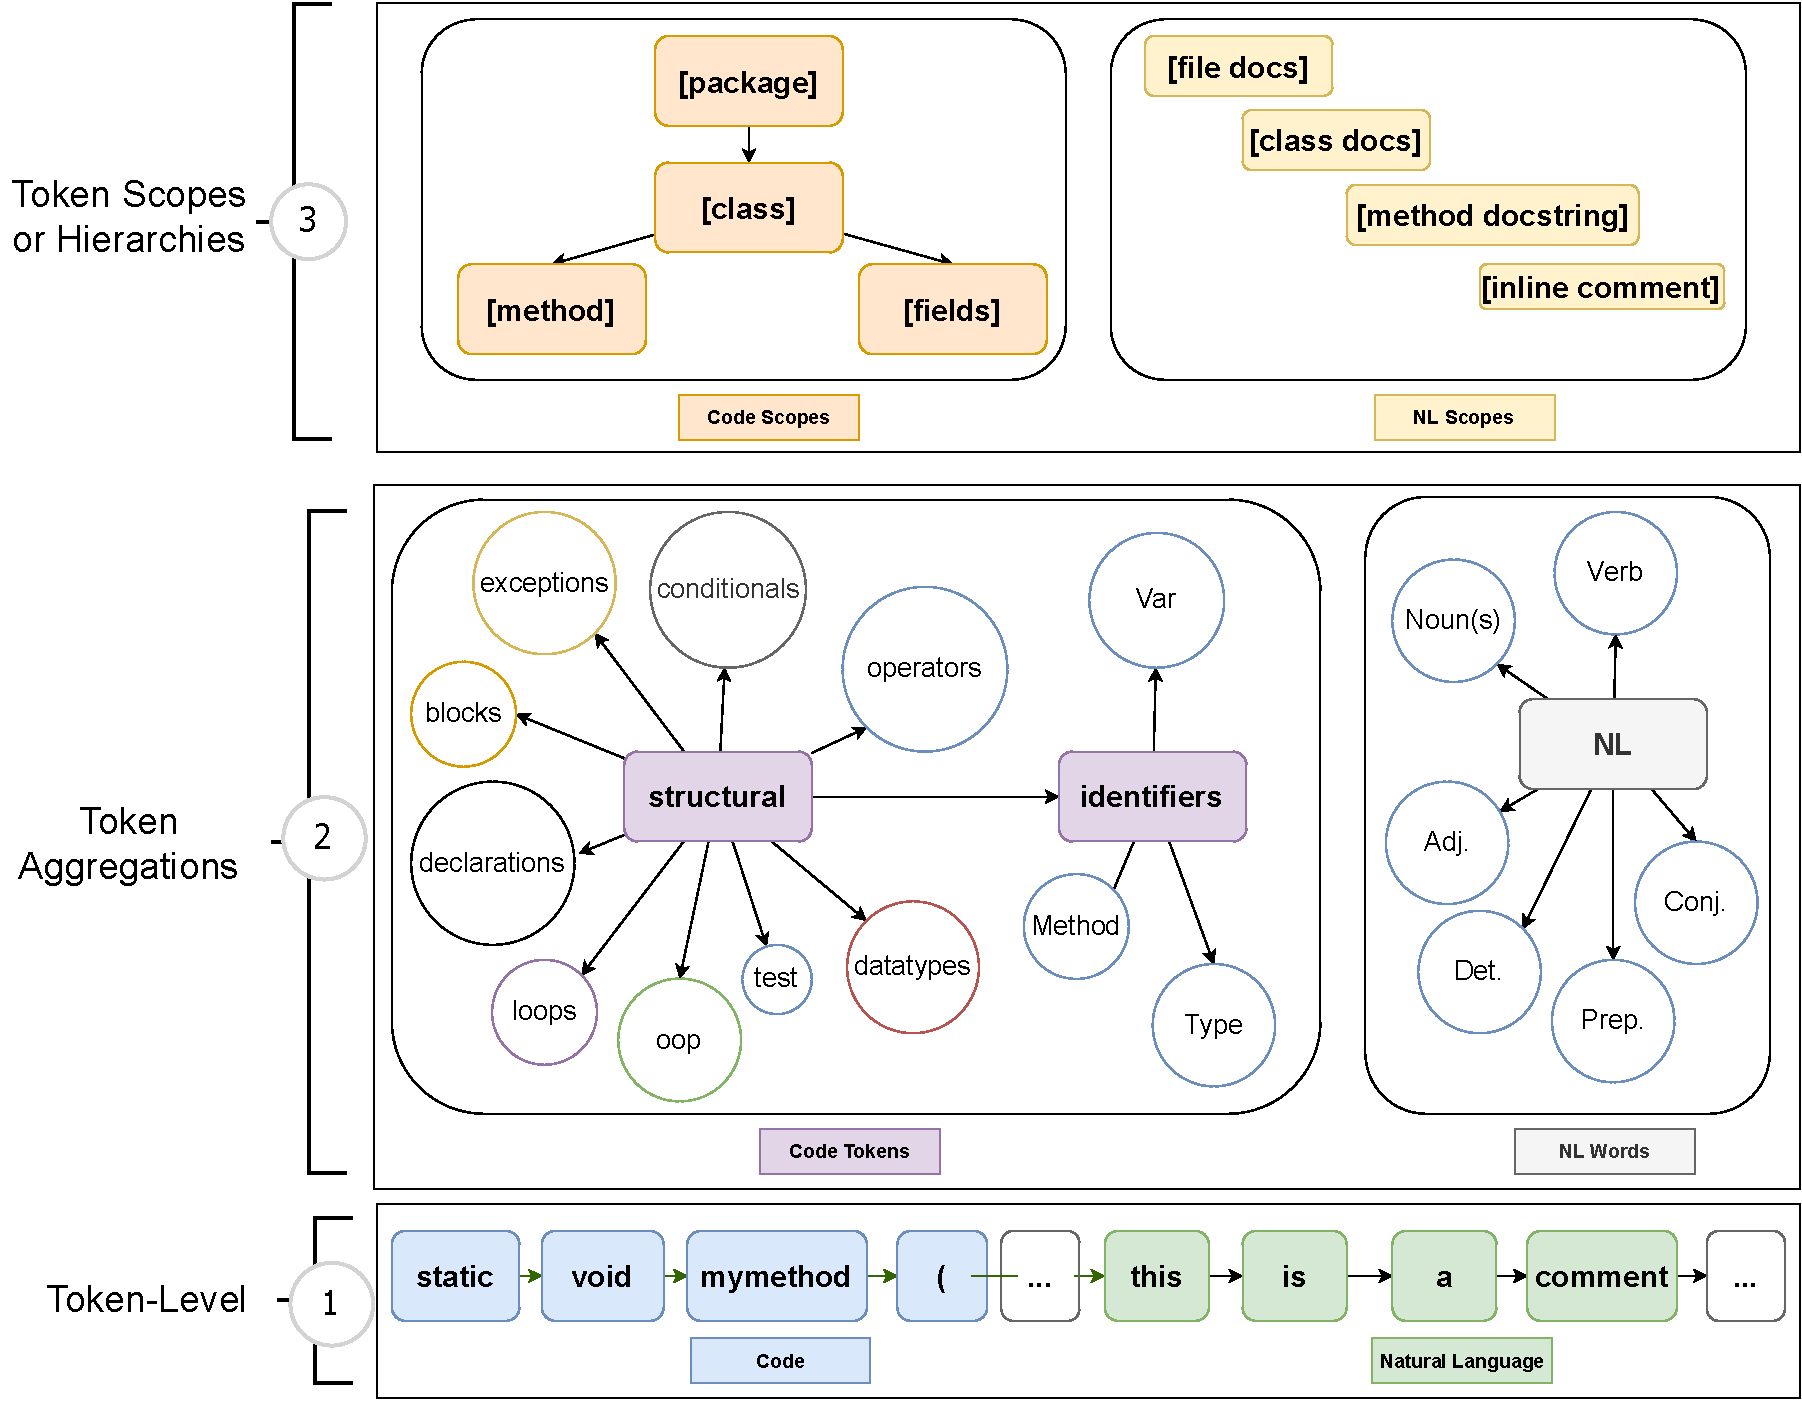
\includegraphics[width=0.9\textwidth]{graphics/chap_08-interpret-rational/fig_1_humanConcepts.pdf}
\label{fig:human}
\end{figure}


\textbf{Complexity Analysis.} In particular, Vafa et al. offer a complexity analysis for the \textit{greedy rationalization} algorithm. The analysis can be segmented in three parts: I) searching the min set of rationales in $m$ steps is $O(m)$; II) searching the max probability of $w'_t$ across $t$ is $O(t)$; and III) computing $F_{\theta}(w_t|w_{<t})$ is quadratic $O(t^2)$, in particular, for transformers. Note that in each step of the greedy rationalization, the term $F_{\theta}(w'_t|w_{r_w})$ must be evaluated, which means a complexity of $O(m^2)$ for a rationale size $m = |r|$. Therefore, if it is assumed that $m < t$, then the greedy rationalization is completed altogether in $O(m^3t)$ steps. Bear in mind that evaluating a transformer for an input $t$ would require $O(t^2)$; greedy rationalization has the same asymptotic complexity as evaluating a transformer if the rationale size $m=t^{1/3}$.

\subsection{Local post-hoc code rationales}

Most NLMs operate upon features, such as a token prediction $P(w_t|h_t)$, that do not \textit{inherently} match high-level concepts a human can easily understand. Such difficulty can be expressed mathematically as representing the state of a machine learning (ML) model as a vector space $\Vec{l}$, which corresponds to data as input features $\mathcal{S} = w_{1:T}$. Conversely, developers operate in a different vector space $\Vec{h}$, which corresponds to a set of human-interpretable concepts $\mathcal{H}$. Interpreting an $P_{\theta}$ model can be formalized as:

\begin{equation}
\phi: \Vec{l} \to \Vec{h}
\label{eq:kim}
\end{equation}

The function $\phi$ is known as \textit{function for interpretability} \citep{Kim2018InterpretabilityTCAV}. This function could adopt many forms (e.g., linear, quadratic, or polynomial) and, therefore, it may not capture all the aspects of its input domain, $\Vec{l} \in \mathcal{S}$, and it may not cover all possible human concepts in $\Vec{h} \in \mathcal{H}$. 

Post-hoc explanations occur after training a code generator $\mathcal{G}_c$. A local post-hoc explanation is the result of the interpretability function $\phi(\mathcal{S},\mathcal{H})$ for a single code sequence $\mathcal{S}$ in terms of \textbf{Human-interpretable concept} $\mathcal{H}$. \equaref{fig:human} shows three levels of human-interpretable concepts: 1) token-level, 2) token aggregations, and 3) token scopes (or hierarchies). In fact, the function \equaref{eq:kim} can be virtually \textit{code rationales} with the form $\phi_0(w_{1:T}, \mathcal{H}^{(0)}) = r(w_{1:T})$ if we consider a rationale a \textit{human-interpretable concept} $\mathcal{H}^{(0)}$. Then, $\phi_0$ would be pure analyses of rationales at token-level. 

However, we could define an extra layer of interpretability beyond reporting tokens within a rationale as depicted in \equaref{fig:human}. Such tokens can be organized or semantically grouped by their function. \equaref{fig:human}-2 presents two-fold aggregation functions depending upon the nature of tokens: code or natural language. Particularly, we proposed a \textit{structural code taxonomy for java} as a first attempt to locally aggregate code rationales $r(\mathcal{S})$ by structural categories (see \equaref{fig:taxonomy}). These categories $\mathcal{H}^{(1)}$ are high-level properties of code that can be mapped from token-level rationales. Using this taxonomy, we are able to interpret NLM predictions in a developer-centric way. In programming languages (PL), different types of tokens retain different semantic meanings. For instance $=$ and $<$ are common \textit{operators}. As such, we can group tokens into semantically meaningful categories that we call \textit{structural concepts} (see \equaref{fig:human}-2). These features will allow us to assign semantic meaning to results when analyzing rationales $r$ by defining 

\begin{equation}
\begin{split}
\phi_1(\mathcal{S}, [\mathcal{H}^{(0)},  \mathcal{H}^{(1)}])  & = \lambda_{\mathcal{H}^{(1)} } ( \phi_0(\mathcal{S}, \mathcal{H}^{(0)} ) \\
                                                            & = \lambda_{\mathcal{H}^{(1)} } ( r(\mathcal{S}) )
\end{split}
\label{eq:structuralagg}
\end{equation}

The mapping function $\lambda_{\mathcal{H}^{(1)}}$ receives a set of rationales of a concrete sequence $\mathcal{S}$ to generate a local explanation in terms of the structural code taxonomy. This explanation is obtained by aggregating rationales by the categories defined in the taxonomy throughout descriptive statistical function (e.g., mean, median, max, etc). Note that new taxonomies for different PLs can be derived/used. The mapping function $\lambda_{\mathcal{H}^{(1)}}$ is, indeed, a parser. This parser could translate or identify categories for a given token (e.g., operators, blocks, or loops) or word (e.g., verb, noun, or adjective). 

We can even go a little bit further and define code concepts by extracting and grouping topics from identifiers (natural language) (see \equaref{fig:human}-2). We refer to these taxonomy as \textbf{Identifier Concepts} $\mathcal{H}^{(2)}$. Here, the mapping function $\lambda_{\mathcal{H}^{(2)}}$ can be defined as an unsupervised approach to generate clusters from semantic embedded in variable names and comments. 



\textbf{Code Context Scopes} $\mathcal{H}^{(3)}$ are other type of suggested taxonomy (see \equaref{fig:human}-3). Oftentimes, it is difficult to predict whether a given NLM will be used in a similar setting to its corresponding sanitized training or testing set. For instance, if a model trained on a well-commented dataset is applied to predict segments of poorly commented code, this could potentially impact performance. As such, we define \textit{Code Context Scopes} to better understand model performance across different hierarchies or levels of context windows.  We formulate these interpretable settings as testbeds (\ie datasets) organized in context scopes. For instance, a testbed oriented to "method scope", may consist of testbeds with such level. Therefore, these datasets describe the Long Range Code Dependency property, which we introduced in the background section. Currently, \codeSeqRational supports both code and natural language scopes. For code scopes $\lambda_{\mathcal{H}^{(3)}}$, four elements are identified: (i) package, (ii) class, (iii) method, and (iv) fields (see \equaref{fig:human}-3). We can also extent the scopes to include signatures or higher level components. We support also custom mapping functions could aggregate tokens at different scopes, highlighting specific parts of the input that are particularly interesting for the downstream task at hand. For example, tokens belonging to a specific method could be aggregated in a specific category (different to other methods), if that method within has a particular role in the taks (\eg a \textit{focal} method for test generation task, a \textit{buggy} method in program repair task).

Following the same logic, other type of categories can be defined in terms of scopes without necessarily implying code hierarchies. We also introduce \textbf{Natural Language-Based Scopes} $\mathcal{H}^{(4)}$ that aggregate code rationales by file docs, class docs, method docstring, and inline comments (see \equaref{fig:human}-3). We may use a distinct mapping function $\lambda_{\mathcal{H}^{(4)}}$ based on code parser as well. 

\subsection{Global post-hoc code rationales}

Global explanations $\Phi(g,\mathcal{S}^n)$ are relevant to understand the overall behavior of a neural language model $\mathcal{G}_c$. We must define an aggregation function $g(\phi,\mathcal{S}^n)$ and a sample $n$ of sequences $\mathcal{S}^n$. Aggregation functions might vary depending on the desired statistical treatment. Even thought, global methods should always describe how input features impact model predictions on average. We suggest, in fact, employing expected values:

\begin{equation}
\Phi(g,\mathcal{S}^n,\mathcal{H}) =  g(\phi_{\mathcal{H}},\mathcal{S}^n) = \frac{1}{n} \sum_{j=1}^{n} \phi_{\mathcal{H}}(\mathcal{S}^j,\mathcal{H})
\label{eq:aggregation}
\end{equation}

Note that global explanations can be tuned for a specific \textit{human-interpretable concept} $\mathcal{H}$. We can observe how, for example, \textit{structural code} categories affect the overall prediction behavior for a given model $\mathcal{G}$. 